\section{Introduzione}
\subsection{Scopo del prodotto}
Lo scopo è quello di fornire uno strumento intuitivo e immersivo per gli utenti che voglio partecipare all'esperienza di esplorare un acquario con i suoi ornamenti e decorazioni.
\newline
Le decorazioni vengono così esposte e visualizzate in un modo molto più autentico e coinvolgente.

\subsection{Descrizione generale}
Per rendere il documento il più esauriente possibile ma allo stesso tempo non troppo prolisso, abbiamo schematizzato ogni caso d'uso evidenziando:  precondizioni, postcondizioni, scenario principale in cui tale azione avrà luogo, una breve descrizione ed eventuali estensioni.\newline
In alcuni casi è stata anche inserita un'immagine dello schema UML per fornire una spiegazione visiva che può aiutare nel comprendere più a fondo il nostro lavoro.\newline

\subsection{Glossario}
In questo documento sono state segnate con il pedice "g" tutte le parole che, secondo noi, necessitano di una spiegazione ulteriore per evitare eventuali ambiguità o incomprensioni. La spiegazione di questi termini la si può trovare nel documento di \textit{Glossario}.

\subsection{Attori}
Data l'ampiezza e struttura ridotta del software, l'attore che interagisce col nostro software è uno solo, denominato "Utente in ambiente 3D". 

\subsubsection{Utente in ambiente 3D}
Si tratta dell'utente protagonista di tutti i casi d'uso del nostro prodotto, chiamato tale dato che il software fornisce un immersione completa all'interno dello scenario 3D. \newline
L'utente non verrà mai reindirizzato a una normale pagina web statica, poiché ne risentirebbe la user experience. 

\pagebreak

\section{Casi d'uso}

\subsection{UC1 - Aggiungere un oggetto al carrello}

\begin{figure}[H]
  \renewcommand{\thefigure}{1}
  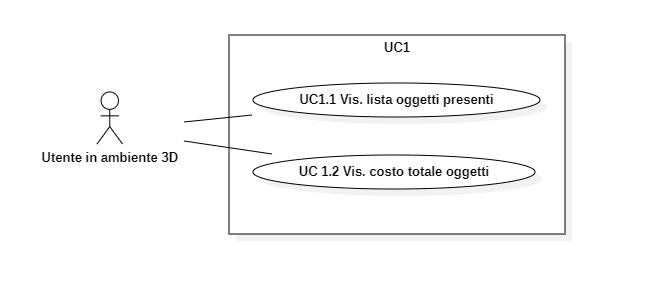
\includegraphics[width=\linewidth]{./res/images/UC1.png}
  \caption{UC1 - Aggiungere un oggetto al carrello}
  \label{fig:UC 1}
\end{figure}

\begin{itemize}

	\item Attore primario: 
	\begin{itemize}
		\item Utente in ambiente 3D.
	\end{itemize}
	\item Descrizione:
	\begin{itemize}
		\item Aggiungere un oggetto al carrello significa aggiungere alla lista degli oggetti presenti nel carrello l'oggetto desiderato e visualizzare un messaggio di oggetto aggiunto al carrello con successo.
\newline L'oggetto all'interno dell'ambiente continua ad esistere anche dopo la sua aggiunta al carrello.
\newline Per inserire una quantità maggiore di una unità di un medesimo oggetto basta aggiungerlo più volte.
	\end{itemize}
	
	\item Precondizioni:
	\begin{itemize}
		\item L'oggetto da aggiungere al carrello si trova all'interno dell'ambiente 3D.
	\end{itemize}
	
	\item Postcondizioni:
	\begin{itemize}
		\item L'oggetto aggiunto al carrello si trova all'interno dell'ambiente 3D;
		\item L'oggetto è presente all'interno del carrello.
	\end{itemize}
	
	\item Scenario principale:
	\begin{itemize}
		\item L'utente interagisce con l'oggetto da aggiungere all'interno del carrello;
		\item L'utente seleziona il comando aggiungi oggetto al carrello.
	\end{itemize}
	
\end{itemize}

\pagebreak

\subsection{UC2 - Visualizzazione contenuto del carrello}

\begin{figure}[H]
  \renewcommand{\thefigure}{2}
  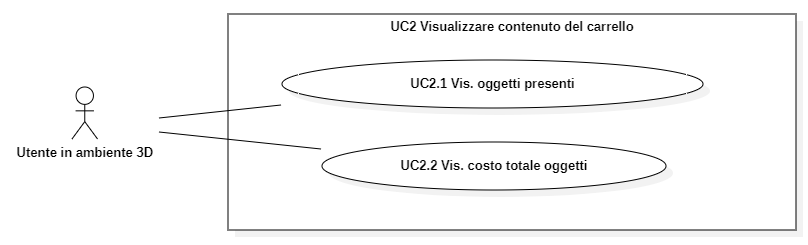
\includegraphics[width=\linewidth]{./res/images/UC2.png}
  \caption{UC2 - Visualizzazione contenuto del carrello}
  \label{fig:UC 2}
\end{figure}

\begin{itemize}
	
	\item Attore primario: 
	\begin{itemize}
		\item Utente in ambiente 3D.
	\end{itemize}
	\item Descrizione:
	\begin{itemize}
		\item Permette di visualizzare il contenuto del carrello.
	\end{itemize}
	
	\item Precondizioni:
	\begin{itemize}
		\item Il contenuto del carrello è nascosto.
	\end{itemize}
	
	\item Postcondizioni:
	\begin{itemize}
		\item Il contenuto del carrello è visibile.
	\end{itemize}
	
	\item Scenario principale:
	\begin{itemize}
		\item L'utente interagisce con il sistema per visualizzare il contenuto del carrello.
	\end{itemize}
	
\end{itemize}

\subsubsection{UC2.1 - Visualizzazione lista oggetti presenti}

\begin{figure}[H]
  \renewcommand{\thefigure}{3}
  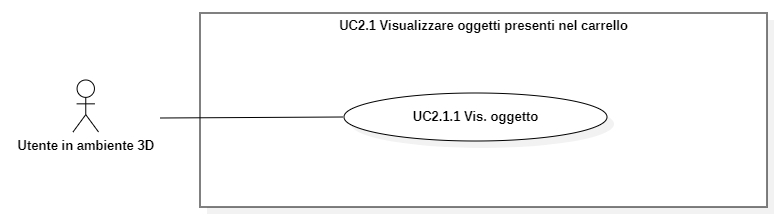
\includegraphics[width=\linewidth]{./res/images/UC2.1.png}
  \caption{UC2.1 - Visualizzazione lista oggetti presenti}
  \label{fig:UC 2.1}
\end{figure}

\begin{itemize}
	
	\item Attore primario: 
	\begin{itemize}
		\item Utente in ambiente 3D.
	\end{itemize}
	\item Descrizione:
	\begin{itemize}
		\item L'utente può visualizzare la lista degli oggetti presenti nel carrello.
	\end{itemize}
	
	\item Precondizioni:
	\begin{itemize}
		\item Il contenuto del carrello è visibile.
	\end{itemize}
	
	\item Postcondizioni:
	\begin{itemize}
		\item Il contenuto del carrello è visibile;
		\item La lista degli oggetti presenti all'interno del carrello è visibile.
	\end{itemize}
	
	\item Scenario principale:
	\begin{itemize}
		\item Nessuna azione richiesta.
	\end{itemize}
	
\end{itemize}

\paragraph{UC2.1.1 - Visualizzazione oggetto}

\begin{figure}[H]
  \renewcommand{\thefigure}{4}
  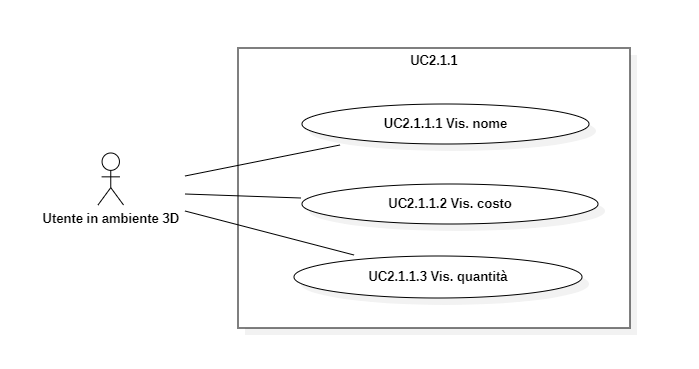
\includegraphics[width=\linewidth]{./res/images/UC2.1.1.png}
  \caption{UC2.1.1 - Visualizzazione oggetto}
  \label{fig:UC 2.1.1}
\end{figure}

\begin{itemize}
	
	\item Attore primario: 
	\begin{itemize}
		\item Utente in ambiente 3D.
	\end{itemize}
	\item Descrizione:
	\begin{itemize}
		\item Prevede la visualizzazione di un oggetto all'interno della lista oggetti del carrello.
	\end{itemize}
	
	\item Precondizioni:
	\begin{itemize}
		\item La lista degli oggetti presenti all'interno del carrello è visibile.
	\end{itemize}
	
	\item Postcondizioni:
	\begin{itemize}
		\item La lista degli oggetti presenti all'interno del carrello è visibile;
		\item L'oggetto è visibile nella lista oggetti del carrello.
	\end{itemize}
	
	\item Scenario principale:
	\begin{itemize}
		\item Nessuna azione richiesta.
	\end{itemize}
	
\end{itemize}

\subparagraph{UC2.1.1.1 - Visualizzazione nome}
\begin{itemize}
	
	\item Attore primario: 
	\begin{itemize}
		\item Utente in ambiente 3D.
	\end{itemize}
	\item Descrizione:
	\begin{itemize}
		\item Prevede la visualizzazione del nome dell’oggetto. Quest'ultimo è considerato come un identificativo che permette di distinguere oggetti diversi tra loro.
	\end{itemize}
	
	\item Precondizioni:
	\begin{itemize}
		\item L'oggetto è visibile nella lista oggetti del carrello.
	\end{itemize}
	
	\item Postcondizioni:
	\begin{itemize}
		\item L'oggetto è visibile nella lista oggetti del carrello;
		\item Il nome associato all'oggetto è visibile.
	\end{itemize}
	
	\item Scenario principale:
	\begin{itemize}
		\item Nessuna azione richiesta.
	\end{itemize}
	
\end{itemize}

\subparagraph{UC2.1.1.2 - Visualizzazione costo}
\begin{itemize}
	
	\item Attore primario: 
	\begin{itemize}
		\item Utente in ambiente 3D.
	\end{itemize}
	\item Descrizione:
	\begin{itemize}
		\item Prevede la visualizzazione del costo dell'oggetto.
	\end{itemize}
	
	\item Precondizioni:
	\begin{itemize}
		\item L'oggetto è visibile nella lista oggetti del carrello.
	\end{itemize}
	
	\item Postcondizioni:
	\begin{itemize}
		\item L'oggetto è visibile nella lista oggetti del carrello;
		\item Il costo associato all'oggetto è visibile.
	\end{itemize}
	
	\item Scenario principale:
	\begin{itemize}
		\item Nessuna azione richiesta.
	\end{itemize}
	
\end{itemize}

\subparagraph{UC2.1.1.3 - Visualizzazione quantità}
\begin{itemize}
	
	\item Attore primario: 
	\begin{itemize}
		\item Utente in ambiente 3D.
	\end{itemize}
	\item Descrizione:
	\begin{itemize}
		\item Prevede la visualizzazione del numero di oggetti identici all'oggetto (compreso) presenti all'interno del carrello.
	\end{itemize}
	
	\item Precondizioni:
	\begin{itemize}
		\item L'oggetto è visibile nella lista oggetti del carrello.
	\end{itemize}
	
	\item Postcondizioni:
	\begin{itemize}
		\item L'oggetto è visibile nella lista oggetti del carrello;
		\item La quantità di oggetti identici all'oggetto (compreso) è visibile.
	\end{itemize}
	
	\item Scenario principale:
	\begin{itemize}
		\item Nessuna azione richiesta.
	\end{itemize}
	
\end{itemize}

\subsubsection{UC2.2 - Visualizzazione costo totale oggetti}

\begin{itemize}
	
	\item Attore primario: 
	\begin{itemize}
		\item Utente in ambiente 3D.
	\end{itemize}
	\item Descrizione:
	\begin{itemize}
		\item Prevede la visualizzazione della somma di tutti i costi degli oggetti presenti all'interno del carrello.
	\end{itemize}
	
	\item Precondizioni:
	\begin{itemize}
		\item Il contenuto del carrello è visibile.
	\end{itemize}
	
	\item Postcondizioni:
	\begin{itemize}
		\item Il contenuto del carrello è visibile;
		\item Il totale della somma di tutti i costi degli oggetti presenti nel carrello è visibile.
	\end{itemize}
	
	\item Scenario principale:
	\begin{itemize}
		\item Nessuna azione richiesta.
	\end{itemize}
	
\end{itemize}


\pagebreak

\subsection{UC3 - Svuotamento totale carrello}

\begin{figure}[H]
  \renewcommand{\thefigure}{5}
  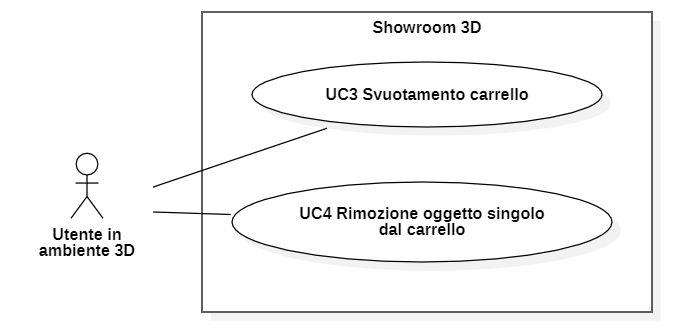
\includegraphics[width=\linewidth]{./res/images/UC3-4.png}
  \caption{UC3 - Svuotamento totale carrello}
  \label{fig:UC 3}
\end{figure}

\begin{itemize}
	
	\item Attore primario: 
	\begin{itemize}
		\item Utente in ambiente 3D.
	\end{itemize}
	\item Descrizione:
	\begin{itemize}
		\item Prevede la rimozione di tutti gli oggetti presenti nel carrello con un singolo comando.
	\end{itemize}
	
	\item Precondizioni:
	\begin{itemize}
		\item Il carrello contiene almeno un oggetto.
	\end{itemize}
	
	\item Postcondizioni:
	\begin{itemize}
		\item Tutti gli oggetti sono stati rimossi dal carrello;
		\item Il carrello è vuoto.
	\end{itemize}
	
	\item Scenario principale:
	\begin{itemize}
		\item L'utente interagisce con il sistema per svuotare completamente il carrello.
	\end{itemize}
	
\end{itemize}

\pagebreak
\subsection{UC4 - Rimozione oggetto singolo dal carrello}

\begin{itemize}
	
	\item Attore primario: 
	\begin{itemize}
		\item Utente in ambiente 3D.
	\end{itemize}
	\item Descrizione:
	\begin{itemize}
		\item Viene rimosso un singolo oggetto dal carrello.
	\end{itemize}
	
	\item Precondizioni:
	\begin{itemize}
		\item Il carrello contiene almeno un oggetto.
	\end{itemize}
	
	\item Postcondizioni:
	\begin{itemize}
		\item Un oggetto è stato rimosso dal carrello.
	\end{itemize}
	
	\item Scenario principale:
	\begin{itemize}
		\item L'utente interagisce con il sistema per la rimozione di un oggetto dal carrello.
	\end{itemize}
	
\end{itemize}

\pagebreak

\subsection{UC5 - Compiere movimenti direzionali}

\begin{figure}[H]
  \renewcommand{\thefigure}{6}
  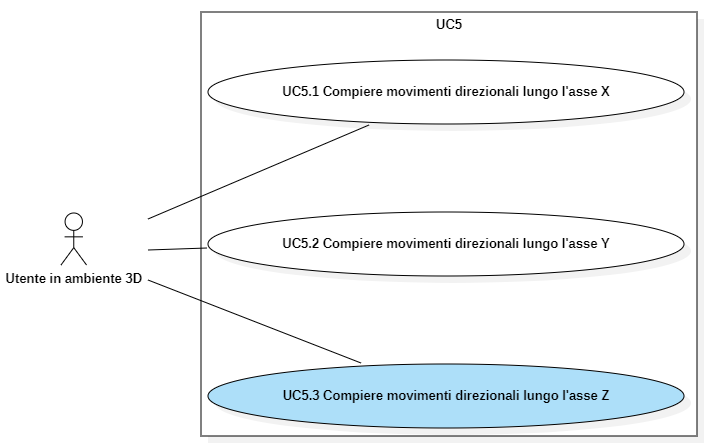
\includegraphics[width=\linewidth]{./res/images/UC5.png}
  \caption{UC5 - Compiere movimenti direzionali}
  \label{fig:UC 5}
\end{figure}

\begin{itemize}

	\item Attore primario: 
	\begin{itemize}
		\item Utente in ambiente 3D.
	\end{itemize}
	\item Descrizione:
	\begin{itemize}
		\item Compiere azioni di movimenti direzionali significa interagire con il sistema per spostarsi nello spazio offerto dall'ambiente 3D.
	\end{itemize}
	
	\item Precondizioni:
	\begin{itemize}
		\item Le azioni di movimento direzionali devono essere abilitate;
		\item Le azioni di movimento direzionali devono essere valide. Un'azione di movimento è considerata valida se l'attore non va a collidere con un oggetto o una parete della stanza;
		\item L'utente si trova in una posizione iniziale nello spazio.
	\end{itemize}
	
	\item Postcondizioni:
	\begin{itemize}
		\item L'utente si trova in una posizione diversa da quella iniziale nello spazio.
	\end{itemize}
	
	\item Scenario principale:
	\begin{itemize}
		\item L'utente interagisce con il sistema per compiere un'azione di movimento direzionale.
	\end{itemize}
	
\end{itemize}


\subsubsection{UC5.1 - Compiere movimenti direzionali lungo l'asse X}
\begin{itemize}

	\item Attore primario: 
	\begin{itemize}
		\item Utente in ambiente 3D.
	\end{itemize}
	\item Descrizione:
	\begin{itemize}
		\item L'attore si sposta in profondità.
	\end{itemize}
	
	\item Precondizioni:
	\begin{itemize}
		\item Le azioni di movimento direzionale lungo l'asse delle X devono essere abilitate;
		\item Le azioni di movimento direzionali lungo l'asse X devono essere valide;
		\item L'utente si trova in una posizione iniziale nello spazio rispetto all'asse X.
	\end{itemize}
	
	\item Postcondizioni:
	\begin{itemize}
		\item L'utente si trova in una posizione diversa da quella iniziale nello spazio rispetto all'asse X.
	\end{itemize}
	
	\item Scenario principale:
	\begin{itemize}
		\item L'utente interagisce con il sistema per compiere un'azione di movimento direzionale lungo l'asse X.
	\end{itemize}
	
\end{itemize}

\subsubsection{UC5.2 - Compiere movimenti direzionali lungo l'asse Y}
\begin{itemize}

	\item Attore primario: 
	\begin{itemize}
		\item Utente in ambiente 3D.
	\end{itemize}
	\item Descrizione:
	\begin{itemize}
		\item L'attore si sposta in orizzontale.
	\end{itemize}
	
	\item Precondizioni:
	\begin{itemize}
		\item Le azioni di movimento direzionale lungo l'asse delle Y devono essere abilitate;
		\item Le azioni di movimento direzionali lungo l'asse Y devono essere valide;
		\item L'utente si trova in una posizione iniziale nello spazio rispetto all'asse Y.
	\end{itemize}
	
	\item Postcondizioni:
	\begin{itemize}
		\item L'utente si trova in una posizione diversa da quella iniziale nello spazio rispetto all'asse Y.
	\end{itemize}
	
	\item Scenario principale:
	\begin{itemize}
		\item L'utente interagisce con il sistema per compiere un'azione di movimento direzionale lungo l'asse Y.
	\end{itemize}
	
\end{itemize}

\subsubsection{UC5.3 - Compiere movimenti direzionali lungo l'asse Z}
\begin{itemize}

	\item Attore primario: 
	\begin{itemize}
		\item Utente in ambiente 3D.
	\end{itemize}
	\item Descrizione:
	\begin{itemize}
		\item  L'attore si sposta in verticale.
	\end{itemize}
	
	\item Precondizioni:
	\begin{itemize}
		\item Le azioni di movimento direzionale lungo l'asse delle Z devono essere abilitate;
		\item Le azioni di movimento direzionali lungo l'asse Z devono essere valide;
		\item L'utente si trova in una posizione iniziale nello spazio rispetto all'asse Z.
	\end{itemize}
	
	\item Postcondizioni:
	\begin{itemize}
		\item L'utente si trova in una posizione diversa da quella iniziale nello spazio rispetto all'asse Z.
	\end{itemize}
	
	\item Scenario principale:
	\begin{itemize}
		\item L'utente interagisce con il sistema per compiere un'azione di movimento direzionale lungo l'asse Z.
	\end{itemize}
	
\end{itemize}

\pagebreak

\subsection{UC6 - Compiere rotazioni camera}

\begin{figure}[H]
  \renewcommand{\thefigure}{7}
  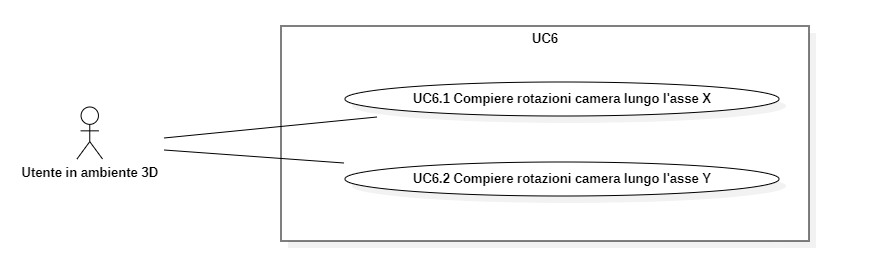
\includegraphics[width=\linewidth]{./res/images/UC6.png}
  \caption{UC6 - Compiere rotazioni camera}
  \label{fig:UC 6}
\end{figure}

\begin{itemize}

	\item Attore primario: 
	\begin{itemize}
		\item Utente in ambiente 3D.
	\end{itemize}
	\item Descrizione:
	\begin{itemize}
		\item Compiere un'azione di rotazione della camera permette all'utente di vedere l'ambiente che lo circonda variando la direzione della propria visuale.
	\end{itemize}
	
	\item Precondizioni:
	\begin{itemize}
		\item L'azione di rotazione della camera deve essere abilitata;
		\item La visuale dell'utente è direzionata verso un punto iniziale.
	\end{itemize}
	
	\item Postcondizioni:
	\begin{itemize}
		\item La visuale dell'utente è direzionata verso un punto diverso rispetto a quello iniziale.
	\end{itemize}
	
	\item Scenario principale:
	\begin{itemize}
		\item L'utente interagisce con il sistema per compiere un'azione di rotazione della camera.
	\end{itemize}
	
\end{itemize}

\subsubsection{UC6.1 - Compiere rotazioni camera lungo l'asse X}
\begin{itemize}

	\item Attore primario: 
	\begin{itemize}
		\item Utente in ambiente 3D.
	\end{itemize}
	\item Descrizione:
	\begin{itemize}
		\item L'attore compie un'azione di rotazione della camera lungo l'asse X.
	\end{itemize}
	
	\item Precondizioni:
	\begin{itemize}
		\item L'azione di rotazione della camera lungo l'asse X deve essere abilitata;
		\item La visuale dell'utente è direzionata verso un punto iniziale.
	\end{itemize}
	
	\item Postcondizioni:
	\begin{itemize}
		\item La visuale dell'utente è direzionata verso un punto nell'asse X diverso rispetto a quello iniziale.
	\end{itemize}
	
	\item Scenario principale:
	\begin{itemize}
		\item L'utente interagisce con il sistema per compiere un'azione di rotazione della camera lungo l'asse X.
	\end{itemize}
	
\end{itemize}

\subsubsection{UC6.2 - Compiere rotazioni camera lungo l'asse Y}
\begin{itemize}

	\item Attore primario: 
	\begin{itemize}
		\item Utente in ambiente 3D.
	\end{itemize}
	\item Descrizione:
	\begin{itemize}
		\item L'attore compie un'azione di rotazione della camera lungo l'asse Y.
	\end{itemize}
	
	\item Precondizioni:
	\begin{itemize}
		\item L'azione di rotazione della camera lungo l'asse Y deve essere abilitata;
		\item La visuale dell'utente è direzionata verso un punto iniziale.
	\end{itemize}
	
	\item Postcondizioni:
	\begin{itemize}
		\item La visuale dell'utente è direzionata verso un punto nell'asse Y diverso rispetto a quello iniziale.
	\end{itemize}
	
	\item Scenario principale:
	\begin{itemize}
		\item L'utente interagisce con il sistema per compiere un'azione di rotazione della camera lungo l'asse Y.
	\end{itemize}
	
\end{itemize}

\pagebreak

\begin{figure}[H]
  \renewcommand{\thefigure}{8}
  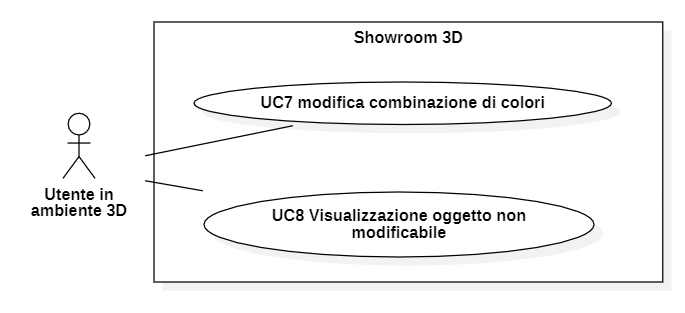
\includegraphics[width=\linewidth]{./res/images/UC7-8.png}
  \caption{UC7 e UC8}
  \label{fig:UC 7-8}
\end{figure}

\subsection{UC7 - Modifica combinazione di colori di un'oggetto}
\begin{itemize}

	\item Attore primario: 
	\begin{itemize}
		\item Utente in ambiente 3D.
	\end{itemize}
	\item Descrizione:
	\begin{itemize}
		\item Modificacombinazione di colori permette all'utente di modificare i colori dell'oggetto con cui sta interagendo.
	\end{itemize}
	
	\item Precondizioni:
	\begin{itemize}
		\item L'oggetto da modificare si trova all'interno dell'ambiente 3D;
		\item L'oggetto da modificare è visibile.
	\end{itemize}
	
	\item Postcondizioni:
	\begin{itemize}
		\item L'oggetto modificato si trova all'interno dell'ambiente 3D;
		\item L'oggetto ha cambiato colori;
	\end{itemize}
	
	\item Scenario principale:
	\begin{itemize}
		\item L'utente interagisce con l'oggetto da modificare;
		\item L'utente seleziona la combinazione di colori tra quelli disponibili;
		\item L'utente apporta le modifiche desiderate;
	\end{itemize}
	
\end{itemize}



\subsection{UC8 - Visualizzazione messaggio oggetto non modificabile}

\begin{itemize}

	\item Attore primario: 
	\begin{itemize}
		\item Utente in ambiente 3D.
	\end{itemize}
	\item Descrizione:
	\begin{itemize}
		\item Prevede la visualizzazione di un messaggio informativo di "oggetto non modificabile".
\newline Un oggetto potrebbe non essere modificabile per la presenza di una sola configurazione per quell'oggetto.
	\end{itemize}
	
	\item Precondizioni:
	\begin{itemize}
		\item L'oggetto da modificare si trova all'interno dell'ambiente 3D;
		\item L'oggetto desiderato non è modificabile.
	\end{itemize}
	
	\item Postcondizioni:
	\begin{itemize}
		\item L'oggetto non è stato modificato;
		\item L'oggetto mantiene le sue caratteristiche visive.
	\end{itemize}
	
	\item Scenario principale:
	\begin{itemize}
		\item L'utente interagisce con l'oggetto da modificare;
		\item L'utente seleziona il comando modifica oggetto.
	\end{itemize}
	
\end{itemize}

\pagebreak

\subsection{UC9 - Visualizzazione lista oggetti della stanza attuale}

\begin{figure}[H]
  \renewcommand{\thefigure}{11}
  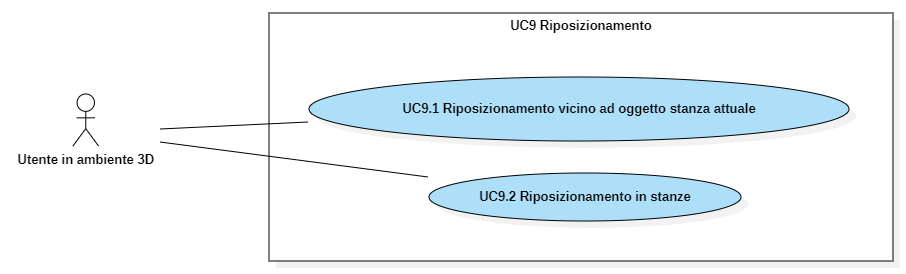
\includegraphics[width=\linewidth]{./res/images/UC9.png}
  \caption{UC9 - Visualizzazione lista oggetti della stanza attuale}
  \label{fig:UC 9}
\end{figure}

\begin{itemize}

	\item Attore primario: 
	\begin{itemize}
		\item Utente in ambiente 3D.
	\end{itemize}
	\item Descrizione:
	\begin{itemize}
		\item Visualizza la lista di tutti gli oggetti presenti nella stanza.
	\end{itemize}
	
	\item Precondizioni:
	\begin{itemize}
		\item Il contenuto della lista oggetti è nascosto.
	\end{itemize}
	
	\item Postcondizioni:
	\begin{itemize}
		\item Il contenuto della lista oggetti è visibile.
	\end{itemize}
	
	\item Scenario principale:
	\begin{itemize}
		\item L'utente interagisce con il sistema per rendere il contenuto della lista oggetti visibile.
	\end{itemize}
	
\end{itemize}


\subsubsection{UC9.1 - Visualizzazione oggetto nella lista}

\begin{figure}[H]
  \renewcommand{\thefigure}{12}
  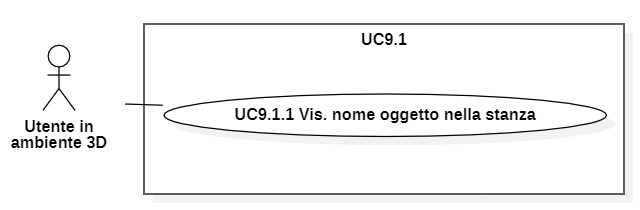
\includegraphics[width=\linewidth]{./res/images/UC9.1.png}
  \caption{UC9.1 - Visualizzazione oggetto nella lista}
  \label{fig:UC 9.1}
\end{figure}

\begin{itemize}

	\item Attore primario: 
	\begin{itemize}
		\item Utente in ambiente 3D.
	\end{itemize}
	\item Descrizione:
	\begin{itemize}
		\item L'utente può vedere un oggetto presente nella lista degli oggetti della stanza corrente.
	\end{itemize}
	
	\item Precondizioni:
	\begin{itemize}
		\item Il contenuto della lista oggetti è visibile.
	\end{itemize}
	
	\item Postcondizioni:
	\begin{itemize}
		\item Il contenuto della lista oggetti è visibile;
		\item L'oggetto è visibile nella lista oggetti.
	\end{itemize}
	
	\item Scenario principale:
	\begin{itemize}
		\item Nessuna azione richiesta.
	\end{itemize}
	
\end{itemize}

\subsubsection{UC9.1.1 - Visualizzazione nome oggetto nella lista}
\begin{itemize}

	\item Attore primario: 
	\begin{itemize}
		\item Utente in ambiente 3D.
	\end{itemize}
	\item Descrizione:
	\begin{itemize}
		\item Prevede la visualizzazione del nome dell’oggetto. Quest'ultimo è considerato come un identificativo che permette di distinguere oggetti diversi tra loro.
	\end{itemize}
	
	\item Precondizioni:
	\begin{itemize}
		\item Il contenuto della lista oggetti è visibile.
	\end{itemize}
	
	\item Postcondizioni:
	\begin{itemize}
		\item Il nome dell'oggetto è visibile nella lista oggetti.
	\end{itemize}
	
	\item Scenario principale:
	\begin{itemize}
		\item Nessuna azione richiesta.
	\end{itemize}
	
\end{itemize}

\pagebreak

\subsection{UC10 - Visualizzazione dettagli oggetto}

\begin{figure}[H]
  \renewcommand{\thefigure}{13}
  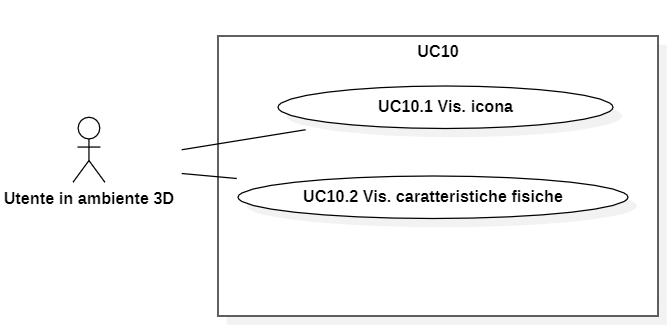
\includegraphics[width=\linewidth]{./res/images/UC10.png}
  \caption{UC10 - Visualizzazione dettagli oggetto}
  \label{fig:UC 10}
\end{figure}

\begin{itemize}
	
	\item Attore primario: 
	\begin{itemize}
		\item Utente in ambiente 3D.
	\end{itemize}
	\item Descrizione:
	\begin{itemize}
		\item L'utente può visualizzarne i dettagli di un oggetto.
	\end{itemize}
	
	\item Precondizioni:
	\begin{itemize}
		\item L'oggetto è visibile.
	\end{itemize}
	
	\item Postcondizioni:
	\begin{itemize}
		\item I dettagli dell'oggetto son visibili.
	\end{itemize}
	
	\item Scenario principale:
	\begin{itemize}
		\item L'utente seleziona un oggetto.
	\end{itemize}
	
\end{itemize}

\begin{figure}[H]
  \renewcommand{\thefigure}{13}
  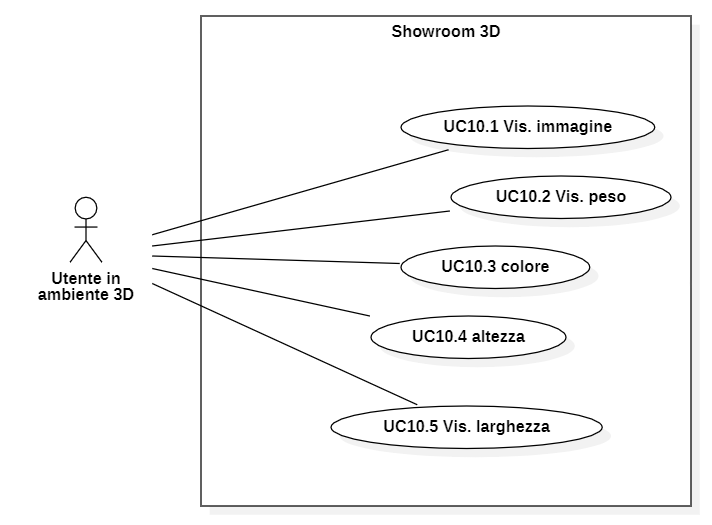
\includegraphics[width=\linewidth]{./res/images/UC10-sottocasi.png}
  \caption{UC10 - Visualizzazione dettagli oggetto}
  \label{fig:UC 10}
\end{figure}

\subsubsection{UC10.1 - Visualizzazione immagine}
\begin{itemize}
	
	\item Attore primario: 
	\begin{itemize}
		\item Utente in ambiente 3D.
	\end{itemize}
	\item Descrizione:
	\begin{itemize}
		\item Prevede la visualizzazione di un'immagine associata all'oggetto a cui fa riferimento.
	\end{itemize}
	
	\item Precondizioni:
	\begin{itemize}
		\item L'oggetto è stato selezionato.
	\end{itemize}
	
	\item Postcondizioni:
	\begin{itemize}
		\item L'immagine associata all'oggetto è visibile.
	\end{itemize}
	
	\item Scenario principale:
	\begin{itemize}
		\item Nessuna azione richiesta.
	\end{itemize}
	
\end{itemize}

\subparagraph{UC10.2 - Visualizzazione peso}
\begin{itemize}

	\item Attore primario: 
	\begin{itemize}
		\item Utente in ambiente 3D.
	\end{itemize}
	\item Descrizione:
	\begin{itemize}
		\item L'utente può vedere il peso dell'oggetto.
	\end{itemize}
	
	\item Precondizioni:
	\begin{itemize}
		\item I dettagli degli oggetti sono visibili.
	\end{itemize}
	
	\item Postcondizioni:
	\begin{itemize}
		\item  I dettagli degli oggetti sono visibili;
		\item L'oggetto è visibile nella lista.
	\end{itemize}
	
	\item Scenario principale:
	\begin{itemize}
		\item Nessuna azione richiesta.
	\end{itemize}
	
\end{itemize}

\subparagraph{UC10.3 - Visualizzazione colore}
\begin{itemize}

	\item Attore primario: 
	\begin{itemize}
		\item Utente in ambiente 3D.
	\end{itemize}
	\item Descrizione:
	\begin{itemize}
		\item L'utente può vedere il colore dell'oggetto.
	\end{itemize}
	
	\item Precondizioni:
	\begin{itemize}
		\item I dettagli degli oggetti sono visibili.
	\end{itemize}
	
	\item Postcondizioni:
	\begin{itemize}
		\item  I dettagli degli oggetti sono visibili;
		\item L'oggetto è visibile nella lista.
	\end{itemize}
	
	\item Scenario principale:
	\begin{itemize}
		\item Nessuna azione richiesta.
	\end{itemize}
	
\end{itemize}

\subparagraph{UC10.4 - Visualizzazione larghezza}
\begin{itemize}

	\item Attore primario: 
	\begin{itemize}
		\item Utente in ambiente 3D.
	\end{itemize}
	\item Descrizione:
	\begin{itemize}
		\item L'utente può vedere la larghezza dell'oggetto.
	\end{itemize}
	
	\item Precondizioni:
	\begin{itemize}
		\item I dettagli degli oggetti sono visibili.
	\end{itemize}
	
	\item Postcondizioni:
	\begin{itemize}
		\item  I dettagli degli oggetti sono visibili;
		\item L'oggetto è visibile nella lista.
	\end{itemize}
	
	\item Scenario principale:
	\begin{itemize}
		\item Nessuna azione richiesta.
	\end{itemize}
	
\end{itemize}

\subparagraph{UC10.5 - Visualizzazione altezza}
\begin{itemize}

	\item Attore primario: 
	\begin{itemize}
		\item Utente in ambiente 3D.
	\end{itemize}
	\item Descrizione:
	\begin{itemize}
		\item L'utente può vedere l'altezza dell'oggetto.
	\end{itemize}
	
	\item Precondizioni:
	\begin{itemize}
		\item I dettagli degli oggetti sono visibili.
	\end{itemize}
	
	\item Postcondizioni:
	\begin{itemize}
		\item  I dettagli degli oggetti sono visibili;
		\item L'oggetto è visibile nella lista.
	\end{itemize}
	
	\item Scenario principale:
	\begin{itemize}
		\item Nessuna azione richiesta.
	\end{itemize}
	
\end{itemize}

\pagebreak

\begin{figure}[H]
  \renewcommand{\thefigure}{16}
  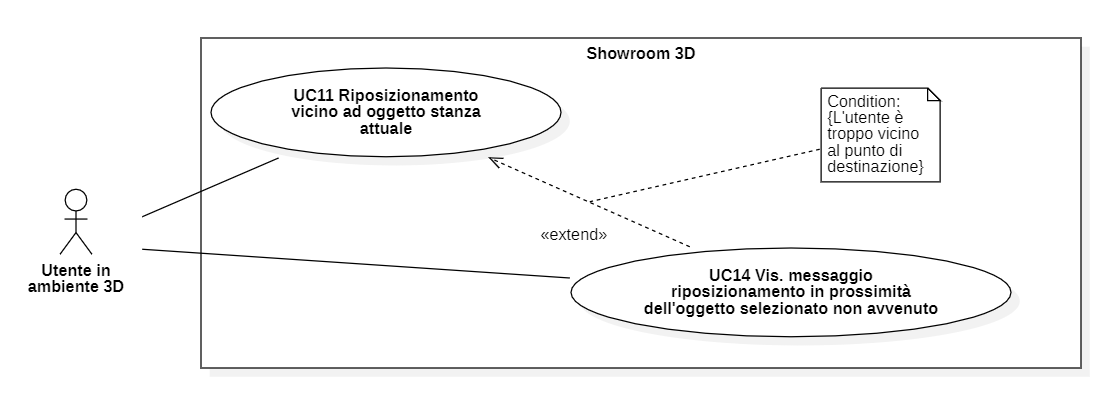
\includegraphics[width=\linewidth]{./res/images/UC11-14.png}
  \caption{UC11 - Riposizionamento vicino ad oggetto stanza attuale}
  \label{fig:UC 11 e UC14}
\end{figure}

\subsection{UC11 - Riposizionamento vicino ad oggetto stanza attuale}
\begin{itemize}

	\item Attore primario: 
	\begin{itemize}
		\item Utente in ambiente 3D.
	\end{itemize}
	\item Descrizione:
	\begin{itemize}
		\item Riposizionamento vicino ad oggetto stanza attuale prevede il riposizionamento dell'utente vicino ad un oggetto
della stanza in cui si trova.
	\end{itemize}
	
	\item Precondizioni:
	\begin{itemize}
		\item L'utente si trova in un punto di partenza.
	\end{itemize}
	
	\item Postcondizioni:
	\begin{itemize}
		\item L'utente si trova nelle vicinanze dell'oggetto desiderato in un punto prestabilito dal sistema.
	\end{itemize}
	
	\item Scenario principale:
	\begin{itemize}
		\item L'utente seleziona il comando per riposizionarsi nelle vicinanze di un oggetto.
	\end{itemize}

	\item Estensioni:
	\begin{itemize}
		\item UC14 - Visualizzazione messaggio riposizionamento in prossimità dell'oggetto selezionato non avvenuto.
	\end{itemize}
	
\end{itemize}

\pagebreak

\begin{figure}[H]
  \renewcommand{\thefigure}{17}
  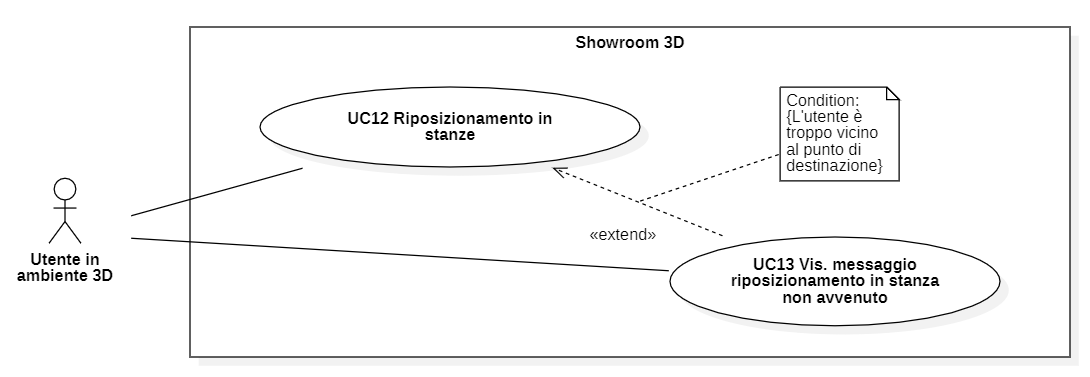
\includegraphics[width=\linewidth]{./res/images/UC12-13.png}
  \caption{UC12 - Riposizionamento in stanze}
  \label{fig:UC 12 e UC13}
\end{figure}

\subsection{UC12 - Riposizionamento in stanze}
\begin{itemize}

	\item Attore primario: 
	\begin{itemize}
		\item Utente in ambiente 3D.
	\end{itemize}
	\item Descrizione:
	\begin{itemize}
		\item Riposizionamento in stanze prevede il riposizionamento dell'utente in un punto prestabilito di una stanza da lui selezionata.
	\end{itemize}
	
	\item Precondizioni:
	\begin{itemize}
		\item L'utente si trova in un punto di partenza di una determinata stanza.
	\end{itemize}
	
	\item Postcondizioni:
	\begin{itemize}
		\item L'utente si trova in un punto prestabilito di una stanza da lui selezionata.
	\end{itemize}
	
	\item Scenario principale:
	\begin{itemize}
		\item L'utente seleziona il comando per riposizionarsi nella stanza desiderata.
	\end{itemize}

	\item Estensioni:
	\begin{itemize}
		\item UC13 Visualizzazione messaggio riposizionamento in stanza non avvenuto.
	\end{itemize}
	
\end{itemize}

\pagebreak

\subsection{UC13 - Visualizzazione messaggio riposizionamento in stanza non avvenuto}
\begin{itemize}

	\item Attore primario: 
	\begin{itemize}
		\item Utente in ambiente 3D.
	\end{itemize}
	\item Descrizione:
	\begin{itemize}
		\item Viene visualizzato un messaggio informativo di riposizionamento in stanza non avvenuto, dopo che l'utente, posizionato ad
una distanza dal punto iniziale della stanza inferiore a quella consentita per il compiersi dell'azione, tenta il ricollocamento in tale stanza.
	\end{itemize}
	
	\item Precondizioni:
	\begin{itemize}
		\item L'utente si trova troppo vicino ad un punto nella stanza da lui selezionata, prestabilito dal sistema, entro la quale non è consentito il ricollocamento;
		\item L'utente interagisce con il comando di riposizionamento in quella destinazione.
	\end{itemize}
	
	\item Postcondizioni:
	\begin{itemize}
		\item Viene visualizzato un messaggio informativo riposizionamento in stanza non avvenuto;
		\item Il riposizionamento non è stato effettuato.
	\end{itemize}
	
	\item Scenario principale:
	\begin{itemize}
		\item Nessuna azione richiesta.
	\end{itemize}
	
\end{itemize}

\pagebreak

\subsection{UC14 - Visualizzazione messaggio riposizionamento in prossimità dell'oggetto selezionato non avvenuto}
\begin{itemize}

	\item Attore primario: 
	\begin{itemize}
		\item Utente in ambiente 3D.
	\end{itemize}
	\item Descrizione:
	\begin{itemize}
		\item Viene visualizzato un messaggio informativo di riposizionamento in prossimità dell'oggetto non avvenuto, dopo che l'utente, posizionato ad
una distanza dall'oggetto inferiore a quella consentita per il compiersi dell'azione, tenta il riposizionamento in prossimità di tale oggetto.
	\end{itemize}
	
	\item Precondizioni:
	\begin{itemize}
		\item L'utente si trova ad una distanza dall'oggetto da lui selezionato entro la quale non è consentito il riposizionamento;
		\item L'utente interagisce con il comando di riposizionamento selezionando l'oggetto che si trova ad una distanza entro la quale non è consentito il riposizionamento.
	\end{itemize}
	
	\item Postcondizioni:
	\begin{itemize}
		\item Il riposizionamento non è avvenuto;
		\item Viene visualizzato un messaggio informativo di riposizionamento in prossimità dell'oggetto non avvenuto.
	\end{itemize}
	
	\item Scenario principale:
	\begin{itemize}
		\item Nessuna azione richiesta.
	\end{itemize}
	
\end{itemize}

\pagebreak

\subsection{UC15 - Visualizzazione lista stanze}

\begin{figure}[H]
  \renewcommand{\thefigure}{18}
  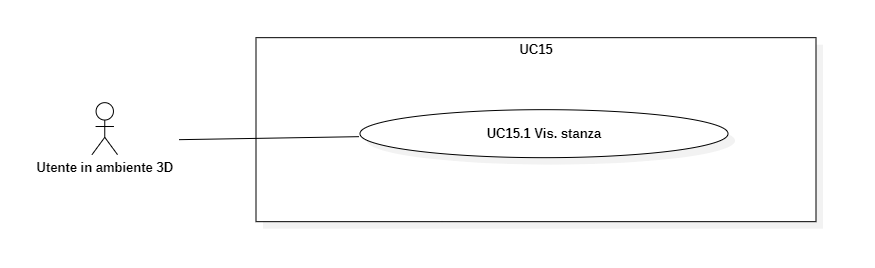
\includegraphics[width=\linewidth]{./res/images/UC15.png}
  \caption{UC15 - Visualizzazione lista stanze}
  \label{fig:UC 15}
\end{figure}

\begin{itemize}

	\item Attore primario: 
	\begin{itemize}
		\item Utente in ambiente 3D.
	\end{itemize}
	\item Descrizione:
	\begin{itemize}
		\item Permette di visualizzare la lista delle stanze, ovvero l'elenco delle stanze presenti all'interno dell'ambiente 3D.
	\end{itemize}
	
	\item Precondizioni:
	\begin{itemize}
		\item La lista delle stanze è nascosta.
	\end{itemize}
	
	\item Postcondizioni:
	\begin{itemize}
		\item La lista delle stanze è visibile.
	\end{itemize}
	
	\item Scenario principale:
	\begin{itemize}
		\item L'utente interagisce con il sistema per rendere la lista delle stanze visibile.
	\end{itemize}
	
\end{itemize}

\subsubsection{UC15.1 - Visualizzazione stanza}

\begin{figure}[H]
  \renewcommand{\thefigure}{19}
  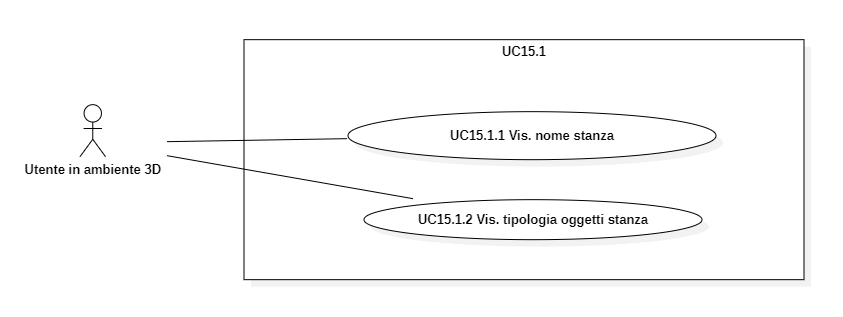
\includegraphics[width=\linewidth]{./res/images/UC15.1.png}
  \caption{UC15.1 - Visualizzazione stanza}
  \label{fig:UC 15.1}
\end{figure}

\begin{itemize}

	\item Attore primario: 
	\begin{itemize}
		\item Utente in ambiente 3D.
	\end{itemize}
	\item Descrizione:
	\begin{itemize}
		\item L'utente visualizza le caratteristiche di una stanza.
	\end{itemize}
	
	\item Precondizioni:
	\begin{itemize}
		\item Il contenuto della lista è nascosto.
	\end{itemize}
	
	\item Postcondizioni:
	\begin{itemize}
		\item Il contenuto della lista è visibile.
	\end{itemize}
	
	\item Scenario principale:
	\begin{itemize}
		\item L'utente interagisce con il sistema per rendere il contenuto della lista visibile.
	\end{itemize}
	
\end{itemize}

\paragraph{UC15.1.1 - Visualizzazione nome stanza}

\begin{itemize}

	\item Attore primario: 
	\begin{itemize}
		\item Utente in ambiente 3D.
	\end{itemize}
	\item Descrizione:
	\begin{itemize}
		\item L'utente visualizza le caratteristiche di una stanza.
		\newline L'utente visualizza il nome della stanza.
	\end{itemize}
	
	\item Precondizioni:
	\begin{itemize}
		\item Il contenuto della lista è visibile.
	\end{itemize}
	
	\item Postcondizioni:
	\begin{itemize}
		\item Il contenuto della lista è visibile;
		\item La stanza è visibile nella lista delle stanze.
	\end{itemize}
	
	\item Scenario principale:
	\begin{itemize}
		\item Nessuna azione richiesta.
	\end{itemize}
	
\end{itemize}


\paragraph{UC15.1.2 - Visualizzazione tipologia oggetti stanza}

\begin{itemize}

	\item Attore primario: 
	\begin{itemize}
		\item Utente in ambiente 3D.
	\end{itemize}
	\item Descrizione:
	\begin{itemize}
		\item L'utente visualizza le caratteristiche di una stanza.
		\newline L'utente visualizza la tipologia di oggetti nella stanza.
	\end{itemize}
	
	\item Precondizioni:
	\begin{itemize}
		\item Il contenuto della lista è visibile.
	\end{itemize}
	
	\item Postcondizioni:
	\begin{itemize}
		\item Il contenuto della lista è visibile;
		\item La stanza è visibile nella lista delle stanze.
	\end{itemize}
	
	\item Scenario principale:
	\begin{itemize}
		\item Nessuna azione richiesta.
	\end{itemize}
	
\end{itemize}

\pagebreak

\begin{figure}[H]
  \renewcommand{\thefigure}{20}
  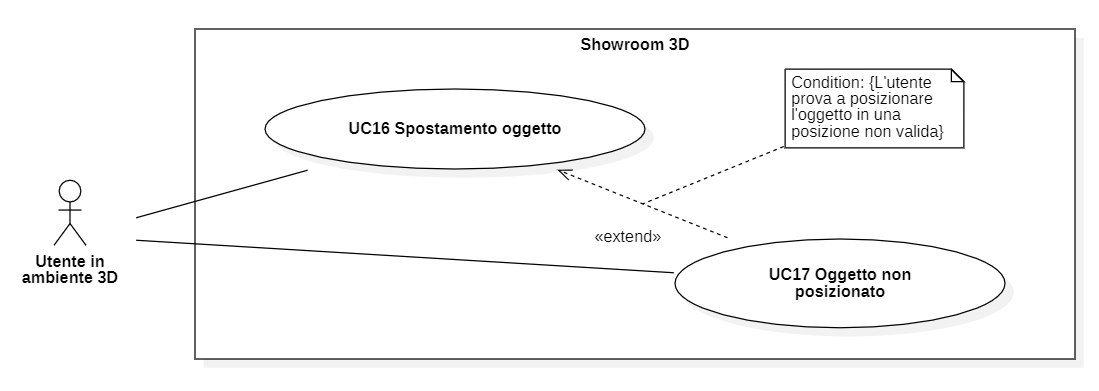
\includegraphics[width=\linewidth]{./res/images/UC16-17.png}
  \caption{UC16 - Spostamento oggetto}
  \label{fig:UC 16 e 17}
\end{figure}

\subsection{UC16 - Spostamento oggetto}
\begin{itemize}

	\item Attore primario: 
	\begin{itemize}
		\item Utente in ambiente 3D.
	\end{itemize}
	\item Descrizione:
	\begin{itemize}
		\item Spostamento di un oggetto in un altro punto della stanza in cui ci si trova.
	\end{itemize}
	
	\item Precondizioni:
	\begin{itemize}
		\item L'oggetto da spostare si trova all'interno dell'ambiente 3D;
		\item L'oggetto si trova in una coordinata X, Y, Z di una stanza.
	\end{itemize}
	
	\item Postcondizioni:
	\begin{itemize}
		\item L'oggetto si trova in una coordinata X, Y, Z diversa da quella di partenza nella stessa stanza.
	\end{itemize}
	
	\item Scenario principale:
	\begin{itemize}
		\item L'utente interagisce con l'oggetto per poterlo spostare in un altra coordinata all'interno della stanza di partenza.
	\end{itemize}
	
	\item Estensioni:
	\begin{itemize}
		\item UC17 - Oggetto non posizionato.
	\end{itemize}
	
\end{itemize}

\pagebreak

\subsection{UC17 - Oggetto non posizionato}
\begin{itemize}

	\item Attore primario: 
	\begin{itemize}
		\item Utente in ambiente 3D.
	\end{itemize}
	\item Descrizione:
	\begin{itemize}
		\item Se l'utente cerca di posizionare un oggetto in una coordinata X, Y, Z non legittima, l'oggetto non viene posizionato.
	\end{itemize}
	
	\item Precondizioni:
	\begin{itemize}
		\item L'oggetto si trova in una coordinata X, Y, Z non valida;
		\item L'oggetto è in fase di spostamento.
	\end{itemize}
	
	\item Postcondizioni:
	\begin{itemize}
		\item L'oggetto è in fase di spostamento;
		\item L'oggetto non è stato posizionato.
	\end{itemize}
	
	\item Scenario principale:
	\begin{itemize}
		\item Nessuna azione richiesta.
	\end{itemize}
	
\end{itemize}

\pagebreak

\subsection{UC18 - Illuminare parte dell'ambiente}
\begin{itemize}

	\item Attore primario: 
	\begin{itemize}
		\item Utente in ambiente 3D.
	\end{itemize}
	\item Descrizione:
	\begin{itemize}
		\item L'utente può illuminare parte dell'ambiente di fronte a lui.
	\end{itemize}
	
	\item Precondizioni:
	\begin{itemize}
		\item L'utente non sta illuminando una parte di ambiente di fronte a lui.
	\end{itemize}
	
	\item Postcondizioni:
	\begin{itemize}
		\item L'utente sta illuminando una parte di ambiente di fronte a lui.
	\end{itemize}
	
	\item Scenario principale:
	\begin{itemize}
		\item L'utente interagisce col sistema per illuminare ciò che si trova di fronte a lui.
	\end{itemize}
	
\end{itemize}

\pagebreak


\section{Requisiti}

\subsection{Introduzione}
Sono stati definiti dei requisiti codificati in base all'ambito di competenza e ad un numero seriale per tenerne meglio traccia, inoltre nelle tabelle sottostanti sono fornite descrizione e classificazione di ciascun requisito.
\tabularnewline
Il codice di ciascuno requisito è formato da:
\begin{itemize}
	\item \textbf{R}: sta per requisito e serve a definire il dominio del codice rendendo subito intuibile che si tratti di un requisito;
	\item Lettera di tipologia:
	\begin{itemize}
		\item \textbf{F}: funzionale;
		\item \textbf{Q}: qualitativo;
		\item \textbf{D}: di dominio;
		\item \textbf{P}: prestazionale.
	\end{itemize}
	\item Numero seriale.
\end{itemize}

\subsection{Requisiti funzionali}
\reqTable{
	\textbf{RF1} & L'utente deve poter aggiungere un oggetto al carrello & Obbligatorio & UC1\tabularnewline
	\textbf{RF2} & L'utente deve poter visualizzare il contenuto del carrello & Obbligatorio & UC2\tabularnewline
	\textbf{RF19} & L'utente deve poter visualizzare un messaggio che indichi se il carrello è vuoto & Facoltativo & UC2 \tabularnewline
     \textbf{RF2.1} & L'utente può visualizzare la lista degli oggetti presenti nel carrello & Obbligatorio & UC2.1\tabularnewline
     \textbf{RF2.2} & L'utente deve poter visualizzare il costo totale degli oggetti presenti nel carrello & Obbligatorio & UC2.2\tabularnewline
     \textbf{RF3} & L'utente deve poter rimuovere tutti gli oggetti dal carrello & Facoltativo & UC3\tabularnewline
	\textbf{RF4} & L'utente deve poter rimuovere un oggetto dal carrello & Facoltativo & UC4 \tabularnewline
     \textbf{RF5} & L'utente deve poter compiere movimenti direzionali & Obbligatorio & UC5\tabularnewline
     \textbf{RF5.1} & L'utente deve poter compiere movimenti direzionali sull'asse X & Obbligatorio & UC5.1\tabularnewline
     \textbf{RF5.2} & L'utente deve poter compiere movimenti direzionali sull'asse Y & Obbligatorio & UC5.2\tabularnewline
     \textbf{RF5.3} & L'utente deve poter compiere movimenti direzionali sull'asse Z & Facoltativo & UC5.3\tabularnewline
     
     \textbf{RF6} & L'utente deve poter compiere spostamenti di camera & Obbligatorio & UC6\tabularnewline
     \textbf{RF6.1} & L'utente deve poter compiere spostamenti di camera lungo l'asse X & Obbligatorio & UC6.1\tabularnewline
     \textbf{RF6.2} & L'utente deve poter compiere spostamenti di camera lungo l'asse Y & Obbligatorio &  UC6.2\tabularnewline
     \textbf{RF7} & L'utente deve poter modificare la combinazione di colori di un oggetto & Obbligatorio & UC7\tabularnewline
     
     \textbf{RF8} & L'utente deve essere notificato in caso un oggetto non fosse modificabile & Obbligatorio & UC8\tabularnewline
     
     \textbf{RF9} & L'utente deve poter visualizzare la lista oggetti della stanza attuale & Facoltativo & UC9\tabularnewline
     \textbf{RF9.1} & L'utente deve poter visualizzare un oggetto nella lista oggetti della stanza attuale & Facoltativo & UC9.1\tabularnewline
     
     \textbf{RF10} & L'utente deve poter visualizzare i dettagli di un oggetto selezionato & Obbligatorio & UC10 \\UC10.1\\UC10.2\\UC10.3\\UC10.4\\UC10.5\tabularnewline

     \textbf{RF11} & L'utente deve poter riposizionarsi vicino ad un oggetto presente nella stanza attuale & Facoltativo & UC11\tabularnewline
     
     \textbf{RF12} & L'utente deve poter riposizionarsi in una stanza da lui selezionata & Facoltativo & UC12\tabularnewline

	\textbf{RF13} & L'utente deve essere notificato quando il riposizionamento in stanza non è concesso & Facoltativo & UC13\tabularnewline
	
	\textbf{RF14} & L'utente deve essere notificato quando il riposizionamento in prossimità di un oggetto selezionato non è concesso & Facoltativo & UC14\tabularnewline 	
	
	\textbf{RF15} & L'utente deve poter visualizzare la lista delle stanze & Facoltativo & UC15\tabularnewline
	\textbf{RF15.1} & L'utente deve poter visualizzare una stanza dalla lista & Facoltativo & UC15.1\tabularnewline
	
	\textbf{RF16} & L'utente deve poter riposizionare un oggetto presente nella stanza attuale & Facoltativo & UC16\tabularnewline
	
	\textbf{RF17} & L'utente non deve poter riposizionare un oggetto in una coordinata non legittima & Facoltativo & UC17\tabularnewline
	
	\textbf{RF18} & L'utente deve poter illuminare l'ambiente davanti a lui & Facoltativo & UC18\tabularnewline
	\textbf{RF20} & L'utente deve poter visualizzare un oggetto con diverse illuminazioni & Obbligatorio & UC18\tabularnewline
	\addlinespace 
	\captionline\caption{Requisiti funzionali}\\}

\subsection{Requisiti qualitativi}
\reqTable{
	\textbf{RQ1} & Il software deve essere sviluppato seguendo le metriche e il modello di qualità descritti nel documento "Norme di Progetto" & Obbligatorio & Decisione interna \tabularnewline
	\textbf{RQ2} & Il software deve essere sviluppato pubblicando il codice sorgente sul repository Github\textsubscript{g} dedicato & Obbligatorio & Decisione interna \tabularnewline
	\textbf{RQ3} & Il software deve essere sviluppato fornendo una documentazione dettagliata delle varie funzionalità & Obbligatorio & Capitolato\tabularnewline
	\textbf{RQ4} & Deve essere fornito un manuale per l’utilizzo& Obbligatorio & Capitolato\tabularnewline
	\textbf{RQ5} & Deve essere fornito un manuale per la manutenzione e l’estensione dell’applicazione& Obbligatorio & Capitolato\tabularnewline	
	\addlinespace 
	\captionline\caption{Requisiti qualitativi}\\}

\subsection{Requisiti di dominio}
\reqTable{
	\textbf{RD1} & Il software deve essere compatibile dalla versione 110 del browser Chrome & Obbligatorio & Decisione interna \tabularnewline
	\textbf{RD2} & Il software deve essere compatibile dalla versione 109 del browser Firefox & Obbligatorio & Decisione interna \tabularnewline
	\textbf{RD3} & Il software deve essere compatibile dalla versione 16 del browser Safari & Obbligatorio & Decisione interna \tabularnewline
	\textbf{RD4} & Il software deve essere compatibile dalla versione 95 del browser Opera & Obbligatorio & Decisione interna \tabularnewline
	\textbf{RD5} & Il software deve essere compatibile dalla versione 110 del browser Microsoft Edge & Obbligatorio & Decisione interna \tabularnewline
	\textbf{RD6} & Il software deve essere sviluppato utilizzando la libreria Three.js & Obbligatorio & Decisione interna\tabularnewline
	\addlinespace 
	\captionline\caption{Requisiti di dominio}\\}

\subsection{Tracciamento}
\subsubsection{Fonte - Requisiti}
\begin{longtable}{ 
		>{\centering}M{0.50\textwidth} 
		>{\centering}M{0.55\textwidth}
		}
	\rowcolorhead
	\headertitle{Fonte} &
	\centering \headertitle{Requisito} 
	\endfirsthead	
	\endhead
	
	Capitolato & RQ3 \\ RQ4 \ RQ5 \tabularnewline
	Decisione interna & RQ1 \\ RQ2 \\ RD1 \\ RD2 \\ RD3 \\ RD4 \\RD5 \\RD6\tabularnewline
	UC1 & RF1\tabularnewline
	UC2 & RF2 \\ RF19 \tabularnewline
	UC2.1 & RF2.1\tabularnewline
	UC2.2 & RF2.2\tabularnewline 
	UC3 & RF3\tabularnewline
	UC4 & RF4 \tabularnewline
	UC5 & RF5 \tabularnewline
	UC5.1 & RF5.1 \tabularnewline
	UC5.2 & RF5.2 \tabularnewline
	UC5.3 & RF5.3 \tabularnewline
	UC6 & RF6 \tabularnewline
	UC6.1 & RF6.1\tabularnewline
	UC6.2 & RF6.2\tabularnewline
	UC7 & RF7 \tabularnewline
	UC8 & RF8 \tabularnewline
	UC9 & RF9 \tabularnewline
	UC9.1 & RF9.1 \tabularnewline
	UC10 & RF10 \tabularnewline
	UC10.1 & RF10 \tabularnewline
	UC10.2 & RF10 \tabularnewline
	UC10.3 & RF10 \tabularnewline
	UC10.4 & RF10 \tabularnewline
	UC10.5 & RF10 \tabularnewline
	UC11 & RF11 \tabularnewline
	UC12 & RF12 \tabularnewline
	UC13 & RF13 \tabularnewline
	UC14 & RF14 \tabularnewline
	UC15 & RF15 \tabularnewline
	UC15.1 & RF15.1\tabularnewline
	UC16 & RF16 \tabularnewline
	UC17 & RF17 \tabularnewline
	UC18 & RF18 \\ RF20 \tabularnewline

\end{longtable}

\subsubsection{Requisiti - Fonti}
\begin{longtable}{ 
		>{\centering}M{0.50\textwidth} 
		>{\centering}M{0.55\textwidth}
		}
	\rowcolorhead
	\headertitle{Requisito} &
	\centering \headertitle{Fonte} 
	\endfirsthead	
	\endhead
	
	RF1 & UC1\tabularnewline
	RF2 & UC2\tabularnewline
	RF2.1 & UC2.1\tabularnewline
	RF2.2 & UC2.2\tabularnewline
	RF3 & UC2\tabularnewline
	RF4 & UC4\tabularnewline
	RF5 & UC5\tabularnewline
	RF5.1 & UC5.1\tabularnewline
	RF5.2 & UC5.2\tabularnewline
	RF5.3 & UC5.3\tabularnewline
	RF6 & UC6\tabularnewline
	RF6.1 & UC6.1\tabularnewline
	RF6.2 & UC6.2\tabularnewline
	RF7 & UC7\tabularnewline
	RF8 & UC8\tabularnewline
	RF9 & UC9\tabularnewline
	RF9.1 & UC9.1\tabularnewline
	RF10 & UC10 \\UC10.1\\UC10.2\\UC10.3\\UC10.4\\UC10.5\tabularnewline
	RF11 & UC11\tabularnewline
	RF12 & UC12\tabularnewline
	RF13 & UC13\tabularnewline
	RF14 & UC14\tabularnewline
	RF15 & UC15\tabularnewline
	RF15.1 & UC15.1\tabularnewline
	RF16 & UC16\tabularnewline
	RF17 & UC17\tabularnewline
	RF18 & UC18\tabularnewline
	RF19 & UC2 \tabularnewline
	RF20 & UC18\tabularnewline
	RQ1 & Decisione interna\tabularnewline
	RQ2 & Decisione interna\tabularnewline
	RQ3 & Capitolato\tabularnewline
	RQ4 & Capitolato\tabularnewline
	RQ5 & Capitolato\tabularnewline
	RD1 & Decisione interna\tabularnewline
	RD2 & Decisione interna\tabularnewline
	RD3 & Decisione interna\tabularnewline
	RD4 & Decisione interna\tabularnewline
	RD5 & Decisione interna\tabularnewline
	RD6 & Decisione interna\tabularnewline
	
\end{longtable}

\subsubsection{Riepilogo Requisiti}
\begin{longtable}{ 
		>{\centering}M{0.25\textwidth} 
		>{\centering}M{0.25\textwidth}
		>{\centering}M{0.25\textwidth}
		>{\centering}M{0.245\textwidth}
		}
	\rowcolorhead
	\headertitle{Tipologia} &
	\centering \headertitle{Obbligatorio} &
	\centering \headertitle{Facoltativo} &
	\centering \headertitle{Totale}  
	\endfirsthead	
	\endhead
	
	Funzionale & 15 & 15& 30\tabularnewline
	Qualitativi & 5 & 0 & 5\tabularnewline
	Dominio & 6 & 0& 6\tabularnewline
	\rowcolorhead \textcolor{white}{\textbf{Tutti requisiti}} & \textcolor{white}{\textbf{26}} & \textcolor{white}{\textbf{15}} & \textcolor{white}{\textbf{45}}
\end{longtable}